\documentclass[11pt,a4paper]{article}
\usepackage[margin=1in]{geometry}
\usepackage{amsmath,amssymb,amsthm,bm}
\usepackage{graphicx,booktabs,siunitx,microtype,hyperref,xcolor}
\usepackage[numbers,sort&compress]{natbib}
\hypersetup{colorlinks=true,linkcolor=blue!60!black,citecolor=blue!60!black,urlcolor=blue!60!black}
\graphicspath{{../results/figs/}}
\newtheorem{theorem}{Theorem}\newtheorem{lemma}[theorem]{Lemma}\newtheorem{proposition}[theorem]{Proposition}
\newtheorem{corollary}[theorem]{Corollary}\theoremstyle{remark}\newtheorem{remark}[theorem]{Remark}
\newcommand{\R}{\mathbb{R}}\newcommand{\C}{\mathbb{C}}\newcommand{\PSD}{\succeq 0}
\DeclareMathOperator{\Tr}{Tr}\DeclareMathOperator{\rank}{rank}\DeclareMathOperator{\conj}{conj}
\newcommand{\I}{I}\newcommand{\rhostar}{\rho^{\star}}

\title{Certified Bounds for Partially Coherent Mask Synthesis:\\ Convex Printability Certificates, Rigorously Separated Single- and Multi-Exposure Optima, and Pattern-Specific Exposure-Latitude Limits}
\author{Autonomous research system (Claude), with human oversight\thanks{Code, data and the full verification record are available in the accompanying repository (\texttt{code/}, \texttt{results/}, \texttt{notes/}). Every number in this manuscript is produced by \texttt{code/run\_all\_par.sh} from scratch.}}
\date{October 12, 2026 --- manuscript v2 (internally verified; not peer reviewed)}

\begin{document}\maketitle

\begin{abstract}
Mask synthesis for projection lithography (inverse lithography, ILT; source--mask optimization, SMO) is nonconvex, and a local optimum carries no information about how far it is from the best achievable image. We show that, for the Abbe/Hopkins model of a periodic cell---scalar or vector (high-NA, polarized), with arbitrary pupil aberrations and any set of focus conditions---the best achievable dark-to-bright intensity ratio $\rhostar$ (equivalently the maximum exposure latitude of a threshold resist) over all masks admits a semidefinite relaxation in the diffraction-order domain whose dual is an elementary certificate: nonnegative weights on dark and bright sample points such that one explicit matrix is positive semidefinite. The certificate is checked independently of the solver (an eigenvalue test with a positive margin and a 50-digit Cholesky factorization), is valid for the continuous constraint set when the sample set contains the edge-offset points, and is made rigorous against solver round-off by a one-parameter bisection. We prove that the relaxation equals the unlimited-multiple-exposure (incoherent superposition) problem, so its gap to the best single mask is exactly the value of multiple exposure; that for symmetric illumination arbitrary complex transmission cannot improve the relaxation; that in one dimension the collected spectra of nonnegative masks form the Carath\'eodory--Toeplitz cone; and that mask pixelation at or above the collected-band count leaves the bound unchanged. To separate single- from multi-exposure optima rigorously we introduce a branch-and-bound certifier for the single-mask problem based on interval bounds of positive semidefinite quadratic forms; it converges in seconds for five collected orders and certifies multi-exposure gains of 6.4--16.4\% on random coherent-illumination targets and 13.4\% on a mixed-width target, independently of the Lasserre moment relaxation that we also report. Across 109 random one-dimensional targets, local optimization is certified globally optimal in 70\% of cases and within 1\% in 83\%; all two-dimensional contact arrays tested under annular, conventional and quasar illumination are certified within 0.3\%; two of three \SI{320}{nm} T-junction and line-end cells are certified within 0.6\%. The bound reproduces the classical $k_1$ cutoffs exactly for DUV and EUV, is 3--150$\times$ tighter than the generalized-eigenvalue (Rayleigh-quotient) bound underlying earlier global heuristics, certifies that binary masks forfeit 3--14\% in ratio relative to phase-shift masks, shows that a standard pattern-error ILT lands 30--67\% above the certified optimum, and survives the vector model and moderate aberrations.
\end{abstract}

\section{Introduction}
Computational lithography synthesizes a mask (and a source) so that the projected aerial image prints a target layout. In the Abbe formulation the image is a weighted sum over source points of squared moduli of filtered mask spectra: it is \emph{quadratic} in the mask. ILT and SMO therefore optimize nonconvex functionals. IBM's wavefront-optimization work states that mask optimization ``tends inherently to be a problem with non-convex quadratic constraints'' \cite{rosenbluth2007}, and recent work on learned ILT describes objectives ``that often trap optimization in poor local minima'' \cite{nvidia2026}; reviews list local optimality among the open problems \cite{pang2021,yang2025}. What is missing is a \emph{certificate}: a proof, for a given target, illumination, numerical aperture and wavelength, that no mask can do better than a stated value. Such certificates (i)~separate unprintable layouts from unconverged optimizers, (ii)~benchmark ILT engines against the true optimum, (iii)~quantify the value of multiple exposure and of phase-shift versus binary masks, (iv)~generalize the $k_1$ rule to arbitrary layouts, and (v)~localize the geometry that limits printability through the support of the dual weights.

\paragraph{Contributions.}
(C1) Theorem~\ref{thm:cert}: dual certificates of printability valid for any mask class and for incoherent sums of masks, verified by one PSD test independent of the solver, with a rigorization procedure (\S\ref{sec:alg}).
(C2) Theorem~\ref{thm:me}: the relaxation equals the unlimited-multi-exposure problem and Pataki's bound limits the number of useful exposures; Lemma~\ref{lem:complex}: complex transmission cannot improve the relaxation under symmetric illumination; Theorem~\ref{thm:toeplitz}: Carath\'eodory--Toeplitz realizability for nonnegative 1D masks; Lemmas~\ref{lem:vector}--\ref{lem:pixel}: vector imaging, aberrations and pixelation preserve the structure.
(C3) Theorem~\ref{thm:bnb}: a rigorous branch-and-bound certificate of the single-mask optimum which, combined with (C1), proves strictly positive multi-exposure gains on concrete targets.
(C4) An open pipeline and an empirical study with independent verification of every certificate.
\paragraph{Not claimed.} No new SDP algorithm (the Shor relaxation of a QCQP is textbook \cite{luo2010,boyd2004}); no full-chip scalability; no thick-mask electromagnetics or resist chemistry; no statement about proprietary ILT engines.

\section{Related work}
\emph{Wavefront optimization.} Rosenbluth et al.\ \cite{rosenbluth2002,rosenbluth2007} optimize the collected diffraction orders directly, maximizing exposure latitude subject to bright/dark intensity constraints; a patent of the same group writes the problem as a quadratic program in the order amplitudes \cite{ibm_patents}. Their global strategies partition the solution space into regions with at most one local minimum \cite{rosenbluth2007}, use dominant ``joint eigenvectors'' and a ``step-walk relaxation'', and, for multiple exposure, an unconstrained Rayleigh-quotient simplification \cite{ibm_patents}. None yields a bound on solutions obtained by other means; we compare with the Rayleigh-quotient bound in Table~\ref{tab:rayleigh}.
\emph{Exact methods for small binary masks.} Liu and Zakhor \cite{liu1992} designed binary and phase-shift masks by branch and bound on a pixel least-squares criterion (combinatorial), whereas Theorem~\ref{thm:bnb} certifies the continuous single-mask optimum of the ratio problem.
\emph{SDP relaxation of QCQPs.} The Shor relaxation and its approximation theory are surveyed in \cite{luo2010}; max-min multicast beamforming \cite{sidiropoulos2006} has exactly the structure of coherent-illumination mask synthesis. Pataki \cite{pataki1998} bounds the rank of extreme solutions; Lasserre's hierarchy \cite{lasserre2001} tightens bounds for small problems.
\emph{Bounds in photonic design.} Angeris, Vu\v{c}kovi\'c and Boyd \cite{angeris2019,angeris2021} bound inverse-designed photonic devices by Lagrangian duality; our work is the imaging-side analogue. SDP relaxations have been used in lithography only for the combinatorial mask-assignment problem of multiple patterning \cite{kohira2016}.
\emph{Information-theoretic limits} \cite{ma2017,wang2018} bound OPC fidelity through mutual information; these are not layout-specific duality certificates. \emph{Lifting in imaging:} PhaseLift \cite{candes2013} lifts quadratic measurements for recovery; we lift for synthesis. The optimal coherent decomposition of partially coherent imaging is due to \cite{pati1994}.

\section{Model and problem}\label{sec:model}
Let $\Lambda=[0,L_1)\times\dots\times[0,L_d)$, $d\in\{1,2\}$, be a periodic cell and $m:\Lambda\to\C$ the mask transmission with Fourier coefficients $M_k=|\Lambda|^{-1}\int_\Lambda m(x)e^{-2\pi i f_k\cdot x}\,dx$, $f_k=(k_1/L_1,\dots)$. Illumination is a finite set of source points $s_j\in\R^d$ (direction cosines, $|s_j|\le\sigma\,\mathrm{NA}$) with weights $w_j>0$, $\sum_j w_j=1$. The pupil is $P_z(g)=\mathbb{1}\{|g|\lambda\le\mathrm{NA}\}\exp\big(i2\pi z(\sqrt{1-|g|^2\lambda^2}-1)/\lambda + iW(g)\big)$ with defocus $z$ and aberration phase $W$. Only the collected orders $K=\{k:|f_k|\le(\mathrm{NA}+\max_j|s_j|)/\lambda\}$, $F=|K|$, contribute; $M\in\C^F$ denotes $(M_k)_{k\in K}$. The Abbe image at $x$ and focus $z$ is
\begin{equation}\label{eq:image}
\I_{M,z}(x)=\sum_{j} w_j\Big|\sum_{k\in K}P_z(f_k+s_j/\lambda)\,M_k\,e^{2\pi i f_k\cdot x}\Big|^2 = M^{\mathsf H}Q_{x,z}M,\qquad Q_{x,z}=\sum_j w_j c_{j,x,z}c_{j,x,z}^{\mathsf H}\PSD .
\end{equation}
A target is specified by finite sample sets $B$ (bright) and $D$ (dark) placed at exactly $\pm\tau$ (edge tolerance) from every target edge plus interior points, and a focus set $Z$. Mask classes: $\mathcal M_\C=\C^F$; real masks $\mathcal M_\R=\{M:M_{-k}=\overline{M_k}\}$ (phase-shift masks); nonnegative masks $\mathcal M_+\subset\mathcal M_\R$ (binary/attenuated). The dark/bright ratio
\begin{equation}
\rho(M)=\frac{\max_{(x,z)\in D\times Z}\I_{M,z}(x)}{\min_{(x,z)\in B\times Z}\I_{M,z}(x)}
\end{equation}
is scale-invariant; for a threshold resist with one dose over the focus set, $\mathrm{EL}(\rho)=(1-\rho)/(1+\rho)$ is the exposure latitude. The synthesis problem and its relaxation are
\begin{align}
(\mathrm P_{\mathcal M})\quad & \rhostar(\mathcal M)=\inf_{M\in\mathcal M\setminus\{0\}}\rho(M)
 = \min\{t:\ M^{\mathsf H}Q_dM\le t\ (d\in D\!\times\! Z),\ M^{\mathsf H}Q_bM\ge1\ (b\in B\!\times\! Z)\},\\
(\mathrm R)\quad & t_R=\min\{t:\ \Tr(Q_dX)\le t\ (d\in D\!\times\! Z),\ \Tr(Q_bX)\ge1\ (b\in B\!\times\! Z),\ X\PSD\ [,\ X=\conj(\Pi X\Pi)]\},\label{eq:R}
\end{align}
where $\Pi$ is the order-flip permutation and the bracketed constraint selects real masks.

\section{Theory}\label{sec:theory}
\begin{theorem}[Certificate]\label{thm:cert}
Let $\mu\ge0$ on $D\times Z$ with $\sum\mu=1$, $\lambda\ge0$ on $B\times Z$, and $S(\mu,\lambda)=\sum_d\mu_dQ_d-\sum_b\lambda_bQ_b\PSD$. Then $\rho(M)\ge\sum_b\lambda_b$ for every $M\in\C^F\setminus\{0\}$ and for every incoherent sum of images $\sum_i\I_{M_i}$. For real masks it suffices that $\tilde S=\mathrm{Re}(U^{\mathsf H}SU)\PSD$ with $U$ a unitary basis of $\mathcal M_\R$.
\end{theorem}
\begin{proof}
Let $\beta=\min_{B\times Z}\I$ and $\delta=\max_{D\times Z}\I$. Then $\delta=\delta\sum_d\mu_d\ge\sum_d\mu_dM^{\mathsf H}Q_dM=M^{\mathsf H}SM+\sum_b\lambda_bM^{\mathsf H}Q_bM\ge\beta\sum_b\lambda_b$. For sums of images apply the same chain termwise. For $M=Ur$, $r\in\R^F$, $M^{\mathsf H}SM=r^{\mathsf T}\tilde Sr$.
\end{proof}
\begin{lemma}[Real structure]\label{lem:real}
$J(M)=\conj(\Pi M)$ is an antilinear involution; $\mathcal M_\R=\mathrm{Fix}(J)$ is a real $F$-dimensional subspace on which the Hermitian form is real. A PSD $X$ satisfies $X=\conj(\Pi X\Pi)$ iff $XJ=JX$; then $X=UYU^{\mathsf H}$ with $Y\in\mathbb S^F_+$ and $\Tr(QX)=\Tr(\tilde QY)$, $\tilde Q=\mathrm{Re}(U^{\mathsf H}QU)$. Hence (R) for real masks is a real SDP of the same size.
\end{lemma}
\begin{theorem}[Relaxation = unlimited multiple exposure]\label{thm:me}
For $\mathcal M\in\{\mathcal M_\C,\mathcal M_\R\}$, $t_R$ equals the optimal ratio of the summed image of any number of incoherently superposed exposures of masks in $\mathcal M$. If (R) has a rank-one optimum then $\rhostar=t_R$ is attained by a single mask; conversely if $\rhostar=t_R$ is attained then (R) has a rank-one optimum. An extreme optimal solution has $\rank X=r$ with $r(r+1)/2\le|D\times Z|+|B\times Z|$, so at most that many exposures are needed.
\end{theorem}
\begin{proof}
$X\PSD\iff X=\sum_{i\le F}M_iM_i^{\mathsf H}$ and $\Tr(QX)=\sum_i M_i^{\mathsf H}QM_i$ is the summed image; Lemma~\ref{lem:real} gives real $M_i$ in the real-structured case. Writing the inequalities with slacks, (R) is a standard-form SDP with $m=|D\times Z|+|B\times Z|$ equalities and block-diagonal cone $(X,\text{slacks},t^+,t^-)$; Pataki's theorem \cite{pataki1998} bounds $\sum_{\text{blocks}}r_b(r_b+1)/2\le m$.
\end{proof}
\begin{remark}
Attainment of $\rhostar$ is not automatic: $\rho$ is scale-invariant and continuous on the unit sphere away from $\{\min_B\I=0\}$, and the infimum may be approached by masks whose bright and dark intensities vanish together; $\rhostar$ is still certified by Theorem~\ref{thm:cert}.
\end{remark}
\begin{theorem}[Nonnegative masks in 1D]\label{thm:toeplitz}
For $d=1$ and $K=\{-K_{\max},\dots,K_{\max}\}$, $M$ is the in-band coefficient vector of a nonnegative measure iff the Toeplitz matrix $T(M)=(M_{a-b})_{a,b=0}^{K_{\max}}\PSD$; if $T(M)\succ0$ it is realized by a bounded, strictly positive function. Hence $\overline{\mathcal M_+}=\{M:T(M)\PSD\}$.
\end{theorem}
\begin{proof}
Necessity: $v^{\mathsf H}T(M)v=|\Lambda|^{-1}\int m(x)|\sum_av_ae^{2\pi iax/L}|^2dx\ge0$. Sufficiency is the Carath\'eodory--Toeplitz theorem \cite{grenander1958}; measures are weak-$*$ limits of bounded nonnegative functions (Fej\'er means). For $T(M)\succ0$ the Levinson--Durbin recursion gives the maximum-entropy autoregressive extension $f(\theta)=\sigma^2/|a(e^{i\theta})|^2$ with $a$ zero-free on the closed disk, matching $M_0,\dots,M_{K_{\max}}$; $f$ is continuous, bounded and bounded away from zero.
\end{proof}
\begin{proposition}[Cutoff]\label{prop:cutoff}
If $L(\mathrm{NA}+\max_j|s_j|)/\lambda<1$ (pitch below $\lambda/((1+\sigma)\mathrm{NA})$) then $Q_{x,z}$ is independent of $x$, $t_R=1$, and uniform $(\mu,\lambda)$ is a certificate. Above this pitch $t_R<1$ for any target with a bright and a dark point.
\end{proposition}
\begin{lemma}[Complex versus real masks]\label{lem:complex}
If $w(-s)=w(s)$ and the pupil is even, then $\tilde M=\conj(\Pi M)$ produces the same image as $M$ for all $x,z$; consequently $t_R(\mathcal M_\C)=t_R(\mathcal M_\R)$ (take $X=\tfrac12(MM^{\mathsf H}+\tilde M\tilde M^{\mathsf H})$).
\end{lemma}
\begin{lemma}[Vector imaging and aberrations]\label{lem:vector}
With the image-side plane wave of direction cosines $(\alpha,\beta,\gamma)$ carrying the mask-side polarization $p$ rotated by the minimal rotation taking $\hat z$ to the propagation direction (for $p=\hat x$: $E=(1-\alpha^2/(1+\gamma),\,-\alpha\beta/(1+\gamma),\,-\alpha)$, Rodrigues' formula \cite{mack_vector}), the image is a sum of rank-one Hermitian forms over channels (source, polarization, field component), so Theorems~\ref{thm:cert}--\ref{thm:me} apply verbatim; Lemma~\ref{lem:complex} extends for reflection-symmetric polarization ensembles since $E_{x,y}(-g)=E_{x,y}(g)$, $E_z(-g)=-E_z(g)$.
\end{lemma}
\begin{lemma}[Pixelation]\label{lem:pixel}
For a mask piecewise constant on $N\ge F$ pixels per period (1D), $M_k=\mathrm{sinc}(k/N)\,\mathrm{DFT}_k(m)$ maps onto $\C^F$, so the pixel-domain and Fourier-domain relaxations coincide for the scale-free ratio problem; $N<F$ can only raise the bound.
\end{lemma}
\begin{remark}[Sampled versus continuous constraints]
The continuous problem has more constraints than the sampled one, so a certificate for the sampled problem is a valid lower bound for the continuous problem. Numerically the interior samples carry zero dual weight and the bound is invariant to interior spacing (\S\ref{sec:robust}).
\end{remark}
\begin{theorem}[Rigorous single-mask lower bound]\label{thm:bnb}
Let $Q_1..Q_m\PSD$ (dark) and $P_1..P_n\PSD$ (bright) be real symmetric and $\rho(r)=\max_iq_i(r)/\min_jp_j(r)$. (i) $\rhostar(\mathcal M_\R)=\min$ over the faces $\Phi_i=\{r:r_i=1,|r_j|\le1\}$. (ii) For a box $\{c+\delta:|\delta_j|\le h_j\}$ and $q(r)=r^{\mathsf T}Qr$ with $Q\PSD$: $q(c)-2|Qc|\cdot h\le q(r)\le q(c)+2|Qc|\cdot h+h^{\mathsf T}|Q|h$. (iii) Hence $\inf_{\text{box}}\rho\ge\mathrm{LB}:=\max_i\max(q_i(c)-2|Q_ic|\cdot h,0)/\min_j(p_j(c)+2|P_jc|\cdot h+h^{\mathsf T}|P_j|h)$, and a branch-and-bound over boxes covering $\bigcup_i\Phi_i$ returns, at any stopping time, a valid lower bound $L=\min_{\text{leaves}}\mathrm{LB}\le\rhostar(\mathcal M_\R)$; on convergence $L\ge(1-\mathrm{tol})\,U$ with $U$ the incumbent.
\end{theorem}
\begin{proof}
(i) scale and sign invariance; (ii) $q(c+\delta)=q(c)+2(Qc)\cdot\delta+\delta^{\mathsf T}Q\delta$ with $0\le\delta^{\mathsf T}Q\delta\le h^{\mathsf T}|Q|h$; (iii) interval arithmetic and the covering argument.
\end{proof}

\section{Algorithms}\label{sec:alg}
\emph{Bound.} Build $Q_{x,z}$ on the edge-offset sample set and solve the real SDP (CLARABEL \cite{clarabel}; SCS \cite{scs} as fallback).
\emph{Rigorization.} Extract duals; let $N$ be the common null space of $S_D=\sum\mu_dQ_d$ and $S_B=\sum\lambda_bQ_b$ (orders invisible to every weighted constraint; on $N$ every form in Theorem~\ref{thm:cert} vanishes identically); find by bisection the largest $c\le1$ with $\lambda_{\min}(S_D-cS_B)\ge10^{-10}\|S_D-cS_B\|$ on $N^\perp$ (if $S_B$ does not vanish on the near-null space of $S_D$, no projection is applied and bisection lowers $c$, to $0$ if needed); report $c\sum\lambda_b$. Independent check: a 50-digit Cholesky factorization of the projected matrix (mpmath).
\emph{Primal.} Gaussian rounding from $X$; analytic-gradient L-BFGS on a log-sum-exp surrogate of $\log\rho$ (common dose across foci); vectorized SLSQP minimax polish; multistart; optimal-face exploration (random PSD objectives over the optimal face) for low-rank optima; explicit two-exposure refinement.
\emph{Single-mask certification.} Theorem~\ref{thm:bnb} (batched boxes; error terms inflated by $1+10^{-9}$, $10^{-12}$ subtracted) and, as corroboration, the Lasserre-2 moment relaxation \cite{lasserre2001}.
\emph{Variants.} SMO relaxation (one PSD block per source point: unlimited exposures with coherent point sources); doubly-nonnegative (DNN) relaxation for nonnegative masks in the pixel domain; complex-mask relaxation; multi-focus; vector and aberrated pupils; pixel-integrated masks.
\emph{Complexity.} $F\approx(2(1+\sigma)\mathrm{NA}L/\lambda)^d$; the SDP has an $F\times F$ matrix variable and $|B|+|D|$ constraints per focus; \SIrange{0.1}{1.5}{s} for $F\le15$, \SIrange{100}{650}{s} for $F=61$ with 1,200 constraints.

\section{Experiments}\label{sec:exp}
Settings: DUV $\lambda=\SI{193}{nm}$, $\mathrm{NA}=1.35$ (coherent; conventional $\sigma\in\{0.5,0.7,0.9\}$; dipole $\sigma\in\{0.7,0.8\}$; annular 0.6/0.9; quasar 0.6/0.9); EUV $\lambda=\SI{13.5}{nm}$, $\mathrm{NA}=0.33$. Edge tolerance $\tau=\SI{8}{nm}$ unless stated. ``Bound'' is always the rigorized certificate value; ``best single mask'' the best feasible real mask found. All tables are generated from the clean reproduction (\texttt{results/RESULTS\_TABLES.md}).

\subsection{Cutoff recovery}
For dense lines the bound is exactly 1 for pitches below $\lambda/((1+\sigma)\mathrm{NA})=\SI{84.1}{nm}$ at $\sigma=0.7$ and drops below 1 immediately above (Fig.~\ref{fig:k1}). In EUV with $\pm\SI{50}{nm}$ focus the \SI{20}{nm} pitch ($k_1=0.244$) is certified unprintable with any mask under both sources; the $\sigma=0.8$ dipole is also certified unprintable at \SI{22}{nm} pitch, while the $\sigma=0.9$ conventional source reaches $\mathrm{EL}=0.36$; all fourteen EUV cases are tight (gap $0.00\%$).

\subsection{One-dimensional feature library}
\begin{table}[t]\centering\small\caption{1D feature library (DUV; $\tau=\SI{8}{nm}$, dense-90: \SI{6}{nm}). Gap $=$ (best single mask $-$ bound)/bound.}\label{tab:1d}
\begin{tabular}{lrrrrrr}\toprule
case & $F$ & foci & bound $\rho$ & max EL & best single $\rho$ & gap\\\midrule
iso-dense, coherent & 9 & 1 & 0.3625 & 0.468 & 0.4741 & 30.8\%\\
mixed, coherent & 7 & 1 & 0.4211 & 0.407 & 0.4787 & 13.7\%\\
iso-dense, $\sigma=0.7$ & 15 & 1 & 0.4691 & 0.361 & 0.4808 & 2.5\%\\
mixed, $\sigma=0.7$ & 11 & 1 & 0.4825 & 0.349 & 0.4836 & 0.2\%\\
iso-dense, dipole 0.8 & 15 & 1 & 0.4313 & 0.397 & 0.4313 & 0.0\%\\
mixed, dipole 0.8 & 13 & 1 & 0.4211 & 0.407 & 0.4211 & 0.0\%\\
iso-dense, $\sigma=0.7$, $\pm\SI{80}{nm}$ & 15 & 3 & 0.8131 & 0.103 & 0.9044 & 11.2\%\\
mixed, $\sigma=0.7$, $\pm\SI{80}{nm}$ & 11 & 3 & 0.8691 & 0.070 & 0.9742 & 12.1\%\\
iso-dense, dipole 0.8, $\pm\SI{80}{nm}$ & 15 & 3 & 0.7686 & 0.131 & 0.8921 & 16.1\%\\
dense 90, $\sigma=0.7$ / dipole / coherent & 9/9/5 & 1 & 0.6428/0.4217/0.4217 & 0.217/0.407/0.407 & = bound & 0.0\%\\
\bottomrule\end{tabular}\end{table}
Dipole and dense-line cases are exactly tight; conventional-illumination gaps are $\le2.5\%$; coherent illumination shows large gaps (iso-dense 30.8\%, mixed 13.7\%) and the three-focus cases 11--16\% (Table~\ref{tab:1d}).

\subsection{Random targets}
On 109 random targets (1--4 segments $\ge\SI{40}{nm}$ in 300--\SI{600}{nm} cells; $\tau=\SI{10}{nm}$) the best single mask matches the certified bound to $10^{-4}$ in 69.7\% of instances, to 1\% in 82.6\% and to 5\% in 91.7\% (median gap $1.8\times10^{-6}$, maximum 17.3\%). Exact tightness is source-dependent (85\% for $\sigma=0.9$, 75\% dipole, 57\% coherent and $\sigma=0.5$); every gap above 5\% has minimal optimal-face rank 2 or 3, consistent with Theorem~\ref{thm:me}.

\subsection{Certified multi-exposure gains}
\begin{table}[t]\centering\small\caption{Rigorous separation of single- and multi-exposure optima (Theorem~\ref{thm:bnb}; $L\le\rhostar(\mathcal M_\R)\le U$).}\label{tab:bnb}
\begin{tabular}{lrrrrrrr}\toprule
case & $F$ & SDP bound & B\&B $L$ & best single $U$ & nodes & converged & certified gain\\\midrule
random 82 (coh.) & 5 & 0.3597 & 0.4061 & 0.4066 & 40,383 & yes & 12.9\%\\
random 91 (coh.) & 5 & 0.6049 & 0.6775 & 0.6782 & 76,027 & yes & 12.0\%\\
random 110 (coh.) & 5 & 0.3464 & 0.4033 & 0.4037 & 17,413 & yes & 16.4\%\\
random 50 (coh.) & 5 & 0.3141 & 0.3343 & 0.3347 & 28,517 & yes & 6.4\%\\
mixed, coherent & 7 & 0.4211 & 0.4776 & 0.4787 & $3.0\times10^7$ & no (0.23\% gap) & 13.4\%\\
\bottomrule\end{tabular}\end{table}
Theorem~\ref{thm:bnb} converges in \SIrange{0.3}{1.6}{s} for $F=5$ and proves the gains of Table~\ref{tab:bnb}; each optimal face has rank 2, so two exposures suffice. The Lasserre-2 single-mask bounds coincide with $U$ to $10^{-6}$ on these instances (cross-checked between CLARABEL, 0.4787045, and SCS, 0.4787037, on the mixed target). For $F=9$ (iso-dense coherent) and $F=11$ (three-focus mixed target) the interval branch-and-bound does not converge within $6\times10^6$ nodes; only Lasserre-2 values (0.4608 and 0.9552, solver status \emph{optimal\_inaccurate}) corroborate gains of 27\% and 9.9\%, which we therefore do not count as certified.

\subsection{Phase-shift versus binary masks; standard ILT}
The DNN relaxation for nonnegative masks gives 0.4266/0.4599/0.3777 against PSM bounds 0.3879/0.4031/0.3671 on the iso-dense/mixed/dense-120 targets ($\sigma=0.7$, $\tau=\SI{10}{nm}$): binary masks forfeit a certified 10\%/14\%/3\%. Pixel- and Fourier-domain PSM relaxations agree to $10^{-5}$. A standard pattern-error ILT (sigmoid resist, open-frame-normalized intensity, threshold 0.3, best of six settings, 1500 Adam steps, gradient verified by finite differences) reaches 0.553/0.672/0.477 (PSM) and 0.579/0.722/0.517 (binary): 30--79\% above the certified optimum; refining the ILT mask on the ratio objective closes the gap on dense-120 (0.3671) and partially elsewhere (0.426, 0.530).

\subsection{Source--mask entitlement}
For the iso-dense target the per-source-point relaxation equals the coherent bound (0.3625) for $\sigma=0.7$ and for a 13-point $\sigma=0.9$ grid, while fixed-source bounds are 0.43--0.51: no illumination supported on these points beats on-axis coherent light for this metric.

\subsection{Two-dimensional layouts}
\begin{table}[t]\centering\small\caption{2D layouts (DUV, NA 1.35). Contacts: $\tau=12/10/8$\,nm for 160/120/100\,nm pitch; T-junction and line-ends: $\tau=\SI{14}{nm}$. ``strong'' = 12-start search with vectorized SLSQP polish.}\label{tab:2d}
\begin{tabular}{lrrrrrr}\toprule
layout & $F$ & bound $\rho$ & max EL & best single $\rho$ & gap & SDP time\\\midrule
contacts 160, annular & 13 & 0.5843 & 0.262 & 0.5861 & 0.30\% & \SI{1.4}{s}\\
contacts 160, $\sigma=0.5$ & 9 & 0.6174 & 0.237 & 0.6177 & 0.04\% & \SI{1.5}{s}\\
contacts 120, annular & 9 & 0.6957 & 0.179 & 0.6962 & 0.07\% & \SI{0.7}{s}\\
contacts 120, quasar & 9 & 0.5740 & 0.271 & 0.5747 & 0.13\% & \SI{0.7}{s}\\
contacts 100, quasar & 5 & 0.8751 & 0.067 & 0.8754 & 0.03\% & \SI{0.5}{s}\\
T-junction 320, annular (strong) & 61 & 0.4387 & 0.390 & 0.4413 & 0.61\% & \SI{410}{s}\\
T-junction 320, quasar (strong) & 61 & 0.3893 & 0.440 & 0.4135 & 6.2\% & \SI{269}{s}\\
line-ends 320, annular (strong) & 61 & 0.5194 & 0.316 & 0.5195 & 0.03\% & \SI{649}{s}\\
\bottomrule\end{tabular}\end{table}
Contact arrays are certified essentially tight with rank-one optima (Table~\ref{tab:2d}, Fig.~\ref{fig:2d}). For the \SI{320}{nm} cells ($F=61$, $\approx$1,200 constraints) the strong search closes the annular T-junction and the line-end gaps to $0.61\%$ and $0.03\%$; the quasar T-junction retains a 6.2\% gap that we could neither close nor certify as a multi-exposure gain (the interval branch-and-bound is out of reach at $F=61$; a two-exposure local refinement did not beat the single mask). The weighted dark matrix has a 4-dimensional common null space (orders invisible to every constraint); the certificate is verified on its complement. On 40 random two-rectangle layouts in 200--\SI{240}{nm} cells (annular, quasar, $\sigma=0.5$; $F=13$--37) the single-mask search matches the bound to $10^{-3}$ in 45\% and to 5\% in 62.5\% of cases; the remaining gaps (up to 26\%, mostly $\sigma=0.5$ and $F=37$) are unresolved upper bounds on the multi-exposure benefit. EUV contact arrays (32--\SI{44}{nm} pitch, $\pm\SI{40}{nm}$ focus) are tight with certified EL from 0.13 to 0.41 (Fig.~\ref{fig:dataset}).

\subsection{Adversarial targets}
Near-cutoff mixed pitches, SRAF-like \SI{20}{nm} spaces, 5\%/95\% duty cycles, alternating widths and three-pitch mixtures (Fig.~\ref{fig:dataset}) are tight under dipole illumination, mostly tight under $\sigma=0.7$, and show 12--37\% gaps under coherent illumination (rank 3--5), the regime where multi-exposure helps most. The isolated \SI{20}{nm} space under coherent or dipole light has certified bound $\approx0$: a phase-edge mask prints an arbitrarily dark narrow line, which the relaxation recognises.

\subsection{Robustness, solver validation and physics sensitivity}\label{sec:robust}
The bound is invariant to interior spacing (0.46907 for 16$\to$\SI{1}{nm}) and monotone in $\tau$ (EL 0.09 at \SI{2}{nm} to 0.74 at \SI{20}{nm}); source quadrature converges (0.513--0.526 for 11--21 points); the Rayleigh-quotient bound is 1--148$\times$ weaker (Table~\ref{tab:rayleigh}); complex- and real-mask relaxations coincide on all nine cases (Lemma~\ref{lem:complex}). Every reported bound was recomputed and its projected certificate matrix factorized by a 50-digit Cholesky (two EUV cases with bound exactly 1 have $S=0$, Prop.~\ref{prop:cutoff}). CLARABEL and SCS agree to median $7\times10^{-9}$; on five near-degenerate random instances (bounds $\le10^{-2}$) SCS is off by up to 0.14 and once negative, which the certificate check exposes. Under the vector model ($n_{\rm resist}=1.7$) TE bounds are 0--4\% below scalar, unpolarized 10--40\% above, TM 70--120\% above (classical TM contrast loss at NA 1.35), with tightness unchanged; aberrations of 0.02--0.1$\lambda$ move the iso-dense bound by 0--7\%; pixelation at $N\ge F$ leaves it unchanged and coarser pixels raise it (+15\% at \SI{50}{nm}, +46\% at \SI{67}{nm}), as Lemma~\ref{lem:pixel} predicts (Fig.~\ref{fig:bnb}).
\begin{table}[t]\centering\small\caption{SDP bound versus the generalized-eigenvalue (Rayleigh-quotient) bound and the complex-mask relaxation.}\label{tab:rayleigh}
\begin{tabular}{llrrrr}\toprule case & source & $F$ & SDP (real) & Rayleigh & SDP (complex)\\\midrule
iso-dense & coherent & 9 & 0.3625 & 0.0668 & 0.3625\\ iso-dense & $\sigma=0.7$ & 15 & 0.4691 & 0.1387 & 0.4691\\ iso-dense & dipole & 15 & 0.4313 & 0.0823 & 0.4313\\
mixed & coherent & 7 & 0.4211 & 0.0028 & 0.4211\\ mixed & $\sigma=0.7$ & 11 & 0.4825 & 0.0343 & 0.4825\\ dense 90 & $\sigma=0.7$ & 9 & 0.6428 & 0.4392 & 0.6428\\
\bottomrule\end{tabular}\end{table}

\begin{figure}[t]\centering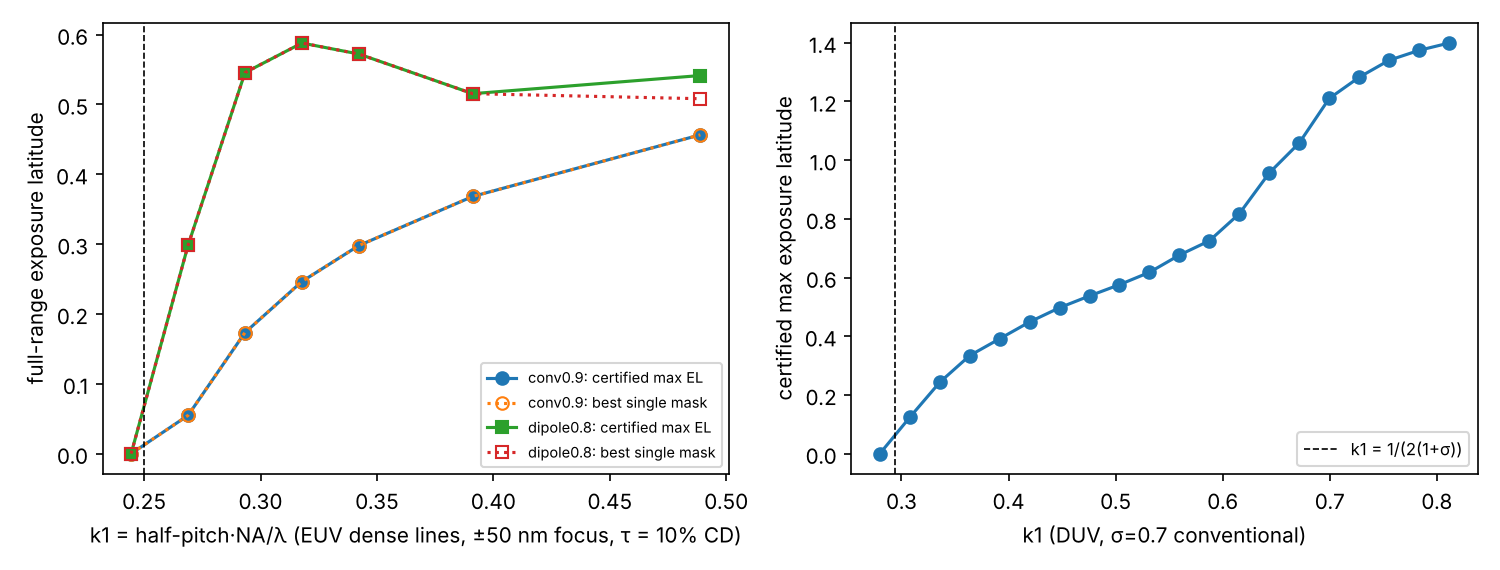
\includegraphics[width=.95\linewidth]{fig2_k1_limits.png}
\caption{Certified maximum exposure latitude versus $k_1$. Left: EUV dense lines with $\pm\SI{50}{nm}$ focus (certified bound and best single mask coincide). Right: DUV, $\sigma=0.7$; dashed line $k_1=1/(2(1+\sigma))$.}\label{fig:k1}\end{figure}
\begin{figure}[t]\centering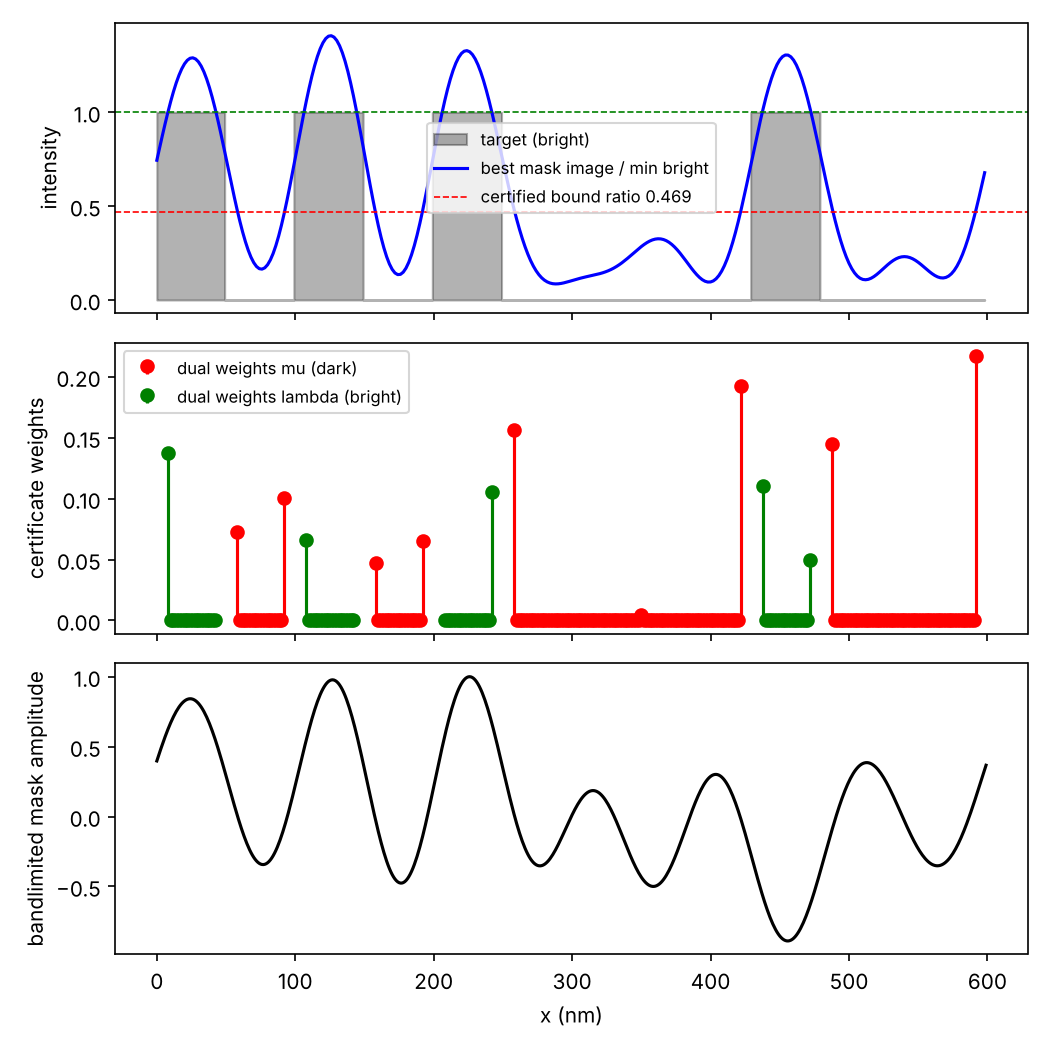
\includegraphics[width=.95\linewidth]{fig1_certificate_isodense.png}
\caption{Iso-dense target ($\sigma=0.7$): best mask image normalized to the minimum bright intensity, dual certificate weights (concentrated on edge-offset points), and the band-limited mask.}\label{fig:cert}\end{figure}
\begin{figure}[t]\centering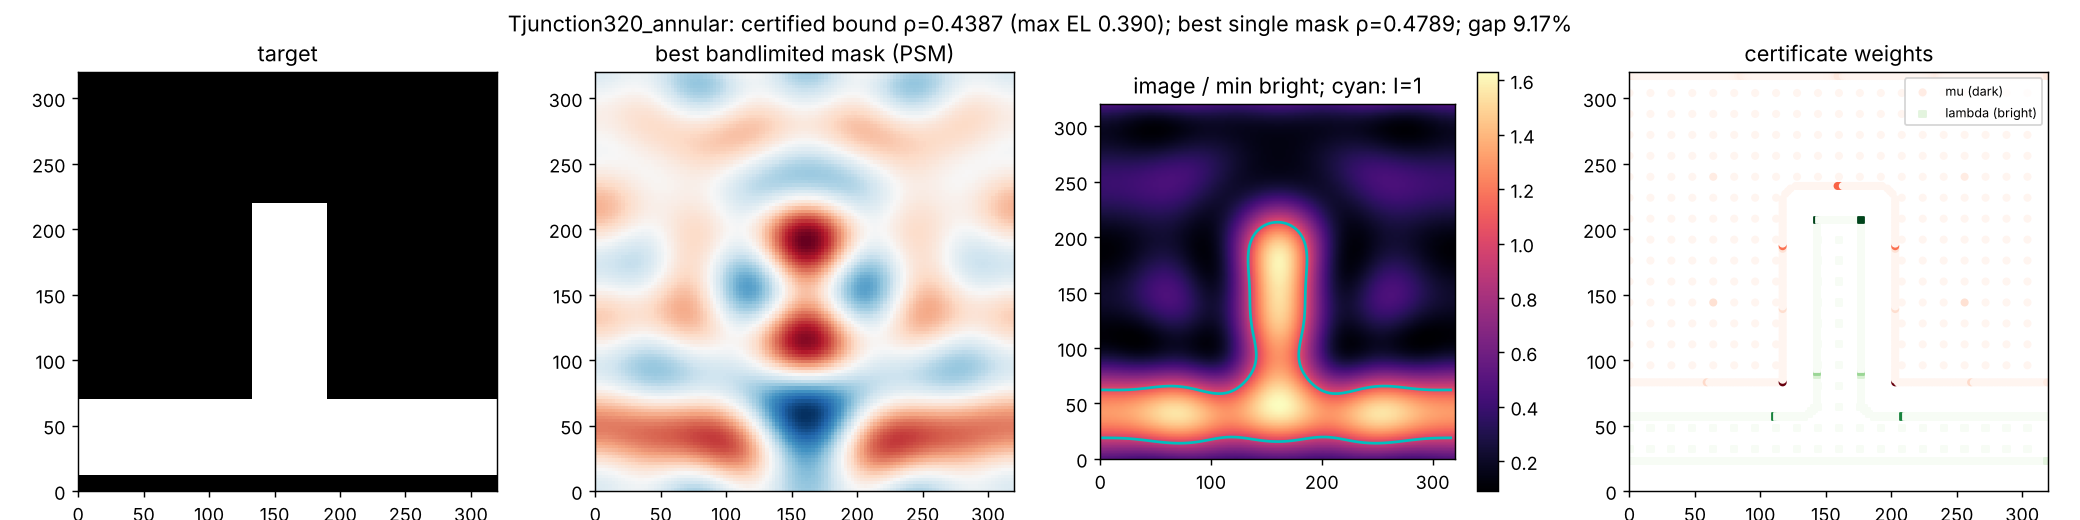
\includegraphics[width=\linewidth]{fig4_2d_Tjunction.png}
\caption{T-junction, annular illumination: target, best band-limited PSM, normalized image with the $\I=1$ contour, and certificate weights localizing the limiting corners and line-end.}\label{fig:2d}\end{figure}
\begin{figure}[t]\centering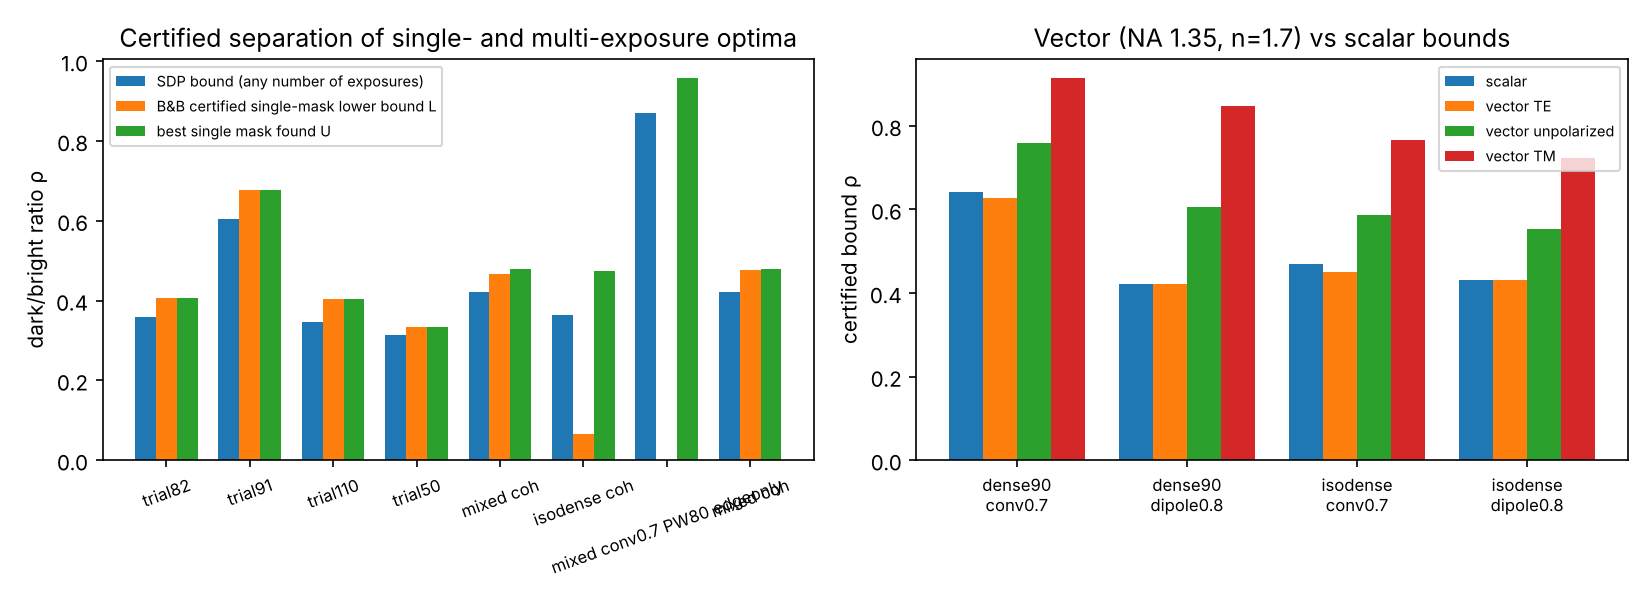
\includegraphics[width=\linewidth]{fig5_bnb_vector.png}
\caption{Left: certified separation of single- and multi-exposure optima (Table~\ref{tab:bnb}). Right: vector versus scalar bounds.}\label{fig:bnb}\end{figure}
\begin{figure}[t]\centering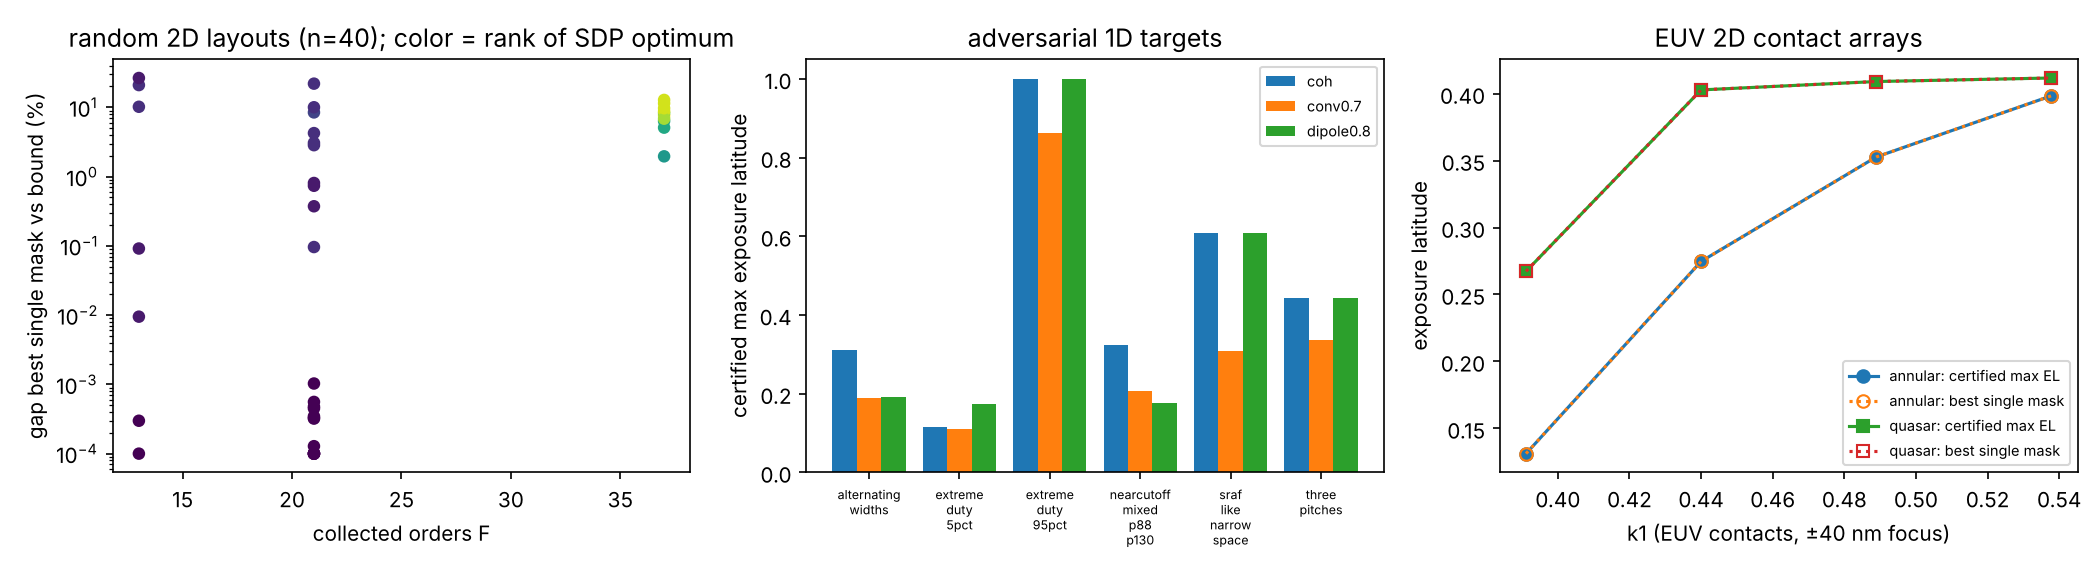
\includegraphics[width=\linewidth]{fig6_dataset.png}
\caption{Expanded dataset: random 2D layouts (gap versus $F$, colour = rank), adversarial 1D targets, EUV 2D contacts.}\label{fig:dataset}\end{figure}

\section{Discussion}
The certificates turn folklore into checkable statements: local optimization of the exposure-latitude objective is globally optimal for most 1D targets and for the 2D contact arrays, and when it is not, the shortfall is---by Theorem~\ref{thm:me}---the benefit of incoherent multiple exposure, which Theorem~\ref{thm:bnb} proves to be strictly positive on concrete coherent-illumination targets; coherent illumination with phase-shift masks is the certified entitlement for the iso-dense target; binary masks forfeit a certified 3--14\%; pattern-error ILT is far from EL-optimal, which argues for EL/contrast objectives or for the certificate as a stopping criterion; and the dual weights localize the limiting geometry. The conclusions survive the vector model and moderate aberrations. The relaxation gap has a physical meaning and is therefore informative rather than merely a weakness.

\section{Limitations}
Thin-mask periodic model (no 3D mask electromagnetics, resist chemistry, flare or mask error); sampled constraints with an explicit edge tolerance; ratio/EL objective (any constraint linear in intensity lifts identically, EPE enters only through $\tau$); the DNN relaxation is only an outer approximation in 2D; Lasserre-2 values carry solver status and are not counted as certificates; the branch-and-bound converges only for $F\le7$; one \SI{320}{nm} 2D gap (6.2\%) and the large-$F$ random 2D gaps remain unresolved; near-degenerate instances (bound $\lesssim10^{-2}$) stress first-order solvers; literature verification relied on abstracts and search snippets (full texts of \cite{rosenbluth2002,rosenbluth2007,liu1992} were not accessible).

\section{Reproducibility}
\texttt{pip install numpy scipy cvxpy matplotlib mpmath}; \texttt{cd code \&\& python3 -W ignore test\_certlitho.py} (9 tests) and \texttt{./run\_all\_par.sh} regenerate every table and figure (about 3.5 hours on four cores). JSON outputs and logs are in \texttt{results/}.

\bibliographystyle{unsrtnat}
\bibliography{refs}
\end{document}
